%\documentclass[12pt]{report}
\documentclass{book}
\usepackage[utf8]{inputenc}
\usepackage{graphicx}
\usepackage{amsmath}
\usepackage{physics}
\usepackage[noBBpl]{mathpazo}
%\usepackage{geometry} \geometry{ a4paper, total={170mm,257mm}, left=20mm, top=20mm,}
%\usepackage{geometry} \geometry{ a4paper, total={170mm,257mm}, left=30mm, right=30mm,}
\usepackage[space]{grffile}
\usepackage{amssymb}
\usepackage{hyperref}	
\usepackage[stable]{footmisc}
\usepackage{amssymb}
\usepackage[nottoc,numbib]{tocbibind}
\usepackage{dsfont}
\usepackage{framed}
\usepackage{caption}
\usepackage{subcaption}
\usepackage{wrapfig}
\usepackage{bm}

\newcommand*\Diff[1]{\mathop{}\!\mathrm{d^#1}}
\newcommand*\erfc{\text{erfc}}
\newcommand{\perr}{\text{p}_{\text{err}}}
\newcommand{\pe}{\text{p}_{\text{e}}}
\newcommand{\given}{\; \middle| \;}
\newcommand{\cond}{\; | \;}
\newcommand{\tmsv}{\rho_{\text{TMSV}}}


\includeonly{
	chapters/introduction,
%	chapters/crypto_intro,
	chapters/qds
}



\DeclareGraphicsExtensions{.pdf,.png,.jpg}


\usepackage{color} 
\def\red#1{\textcolor{red}{#1}}
\def\blue#1{\textcolor{blue}{#1}}
\def\MT#1{\textcolor{magenta}{#1}}
\def\cyan#1{\textcolor{cyan}{#1}}

\graphicspath{ {images/} }

%\setcounter{tocdepth}{1} % Show sections
%\setcounter{tocdepth}{2} % + subsections
\setcounter{tocdepth}{3} % + subsubsections
%\setcounter{tocdepth}{4} % + paragraphs
%\setcounter{tocdepth}{5} % + subparagraphs


\begin{document}
%\part{Secure quantum networks}
%\chapter{Introduction to quantum cryptography}

\section{Conventional (classical) cryptography}
%introduction and literature review
Goal of chapter: historical overview of development of quantum cryptography. Lead up to a thorough literature review for QDS, QSS and QKD.

Cryptography is a field probably as old as civilization itself. For as long as communication has existed, so too has the desire to keep information hidden. Both the Greeks and the Romans are known to have used ciphers to encrypt messages \MT{cite}. A cipher, after applied to a message, alows the encrypted message to be freely transmitted and intercepted without an adverse party knowing its meaning. The intended recipients, however, can undo the effects of the cipher and read the original message. \MT{It'd be cool to have an example of e.g. a ceasar cipher}.

Cryptanalysis--the art and science of breaking cryptographic systems--has existed for as long as cryptography. The history of cryptographic development can be viewed as a race between cryptographers and cryptanalysts. The cryptographers, Alice and Bob, continually invent new schemes to perform their secure communication task. The cryptanalyst, Eve, continually tries to break these schemes in order to interfere in Alice and Bob's communication.

\MT{The following segue seems quite abrupt}
There are two main important strands of cryptography: private-key and public-key crytography, Fig.~\ref{fig:pubpriv}. In private-key cryptography (also known as \emph{symmetric} cryptography), Alice and Bob share some secret information which they will use to perform some task, and without which an eavesdropper cannot break the system. An important example of private-key cryptography is encryption with a cipher $\mathcal{K}$ which is used to encrypt and decrypt messages. Any party with $\mathcal{K}$ can freely encypt or decrypt any piece of information, while any party lacking knowledge of $\mathcal{K}$ cannot. A relevant example of this type of cryptosystem is the one-time pad (OTP) which is discussed above.

\MT{Perhaps some discussion about how $\mathcal{K}$ can be distributed and attacked}

\MT{I should have a discussion at some point about how public- and private- key cryptography relate to each other and how they are both used in modern infrastructure}

The second strand is public-key cryptography (also known as \emph{asymmetric} cryptography). Here, there are several pieces of information required to run a protocol. Alice is assumed to hold a key $\mathcal{E}$ (her ``private key'') while Bob holds a key $\mathcal{D}$ (Alice's ``public-key'') which is assumed to be publicly known. As an example, Alice may encrypt a message using $\mathcal{E}$ and sends it to Bob, who may decrypt it using $\mathcal{D}$.  \MT{Include more examples of this thing actually being used in practice}

\begin{figure}[htp]
\centering
\captionsetup{width=0.8\linewidth}
\begin{framed}
\begin{subfigure}{0.4\textwidth}
\begin{align*}
m \mapsto \text{Encrypt}_\mathcal{K}\left(m\right) \\
\text{Decrypt}_\mathcal{K}\left[E_\mathcal{K}\left(m\right)\right] \mapsto m
\end{align*}
\caption{}
\end{subfigure}
\begin{subfigure}{0.4\textwidth}
\begin{align*}
m \mapsto \text{Encrypt}_\mathcal{E}\left(m\right) \\
\text{Decrypt}_\mathcal{D}\left[\text{Encrypt}_\mathcal{E}\left(m\right)\right] \mapsto m
\end{align*}
\caption{}
\end{subfigure}
\caption{(a) Private-key encryption. The same key $\mathcal{K}$ allows Alice to encrypt and Bob to decrypt message $m$. (b) Public-key encryption. Alice and Bob use different keys, $\mathcal{E}$ and $\mathcal{D}$ to encrypt and decrypt $m$. The decyption key $\mathcal{D}$ can be public knowledge without affecting the security of the encryption key $\mathcal{E}$.}
\label{fig:pubpriv}
\end{framed}
\end{figure}

Usually, given knowledge of $\mathcal{E}$ it should be easy to derive $\mathcal{D}$. The converse should not be true, and the publicly available $\mathcal{D}$ should give no indication of $\mathcal{E}$. If $\mathcal{E}$ is unique to Alice, then a successful decryption using $\mathcal{D}$ proves sufficient to prove Alice's identity.\footnote{One may be tempted to build a digital signatures protocol on this exchange, but \MT{explain why it is a bad idea, with reference to Simmons}.}

The function $f: \mathcal{E} \mapsto \mathcal{D}$ is sometimes referred to as a ``trapdoor'' or ``one-way'' function, and $f$ is typically based on a mathematical problem which is deemed to be computationally hard, for example \MT{examples} which underly the commonly used \MT{protocols}. \MT{motivate quantum cryptography via breaking of these trapdoors}


\section{Quantum digital signatures protocols}
%This section will basically be my "literature review" section.
%I will focus on the main thread of QDS developments initially, but I can supplement it by including some of the asian papers later.

%Note: after I have this section I can compare it to the Amiri2015 review paper and to Collins2018 progress report (and to Callum's thesis)


\subsection*{Quantum one-way function}
%Talk about Gottesman and Chuang.
Gottesman and Chuang \cite{Gottesman2001} generalized Lamport's scheme \MT{cite} in $2001$ to build the first Quantum Digital Signatures protocol. The key contribution of their scheme is to replace the one-way function in \MT{cite} with a so-called \emph{quantum one-way function}, thereby securing the signatures protocol against a quantum adversary.

\MT{TODO: chat more about quantum one-way function. Include the "figure" that I currently have in my historical introduction}

A direct analogue of public-key cryptography, their protocol relies on the difficult task, described in Fig.~\MT{X}, of accurately distinguishing between non-orthogonal quantum states. Their security relies on the fact that performing measurement on a state of $n$~qubits can yield at most $n$~bits of information, and so the protocol in Ref.~\cite{Gottesman2001} is designed such that this is insufficient to distinguish between states.

The key tool in the protocol is a quantum $SWAP$ test, Fig.~\MT{X}, which probabilistically determines whether two states are identical. To perform this test, players prepare $\ket{f_x}, \ket{f_{x^\prime}}$ and an additional ancilla $\left(\ket{0} + \ket{1}\right)/\sqrt{2}$. Players perform a Fredkin gate \MT{cite} using the ancilla as a control, and then perform a Hadamard \MT{cite} on the ancilla. In other words, the $SWAP$ test performs the mapping
\begin{equation}
\ket{f_x}\ket{f_{x^\prime}}\frac{\left(\ket{0} + \ket{1}\right)}{\sqrt{2}} \mapsto \frac{\left(\ket{f_x}\ket{f_{x^\prime}} \pm \ket{f_{x^\prime}}\ket{f_x}\right)\ket{y_{\pm}}}{\sqrt{2}}
\end{equation}
with $y_+=0$ and $y_-=1$. Finally, the ancilla qubit is measured in the $0, 1$ basis, and since $\ket{0}, \ket{1}$ are orthogonal they can be distinguished.  Therefore if $x = x^\prime$ the coefficient of $\ket{1}$ is identically zero, and so the $SWAP$ test always outputs $\ket{0}$. If $x \ne x^\prime$ outputs either $\ket{1}$ or $\ket{0}$. 

The probabilistic nature of this test will cause participants in the protocol to sometimes mistake distinct states for identical ones, but the probability that this occurs may be estimated. Crucially, the protocol may be proven secure if states are chosen such that this probability of honest failure is smaller than the probability to correctly distinguish between large entangled states of non-orthogonal qubits. 

The protocol is a significant attempt to generalise and translate structures from the field of classical cryptography to the quantum realm, and it sets the pattern for all subsequent QDS protocols, and so it is worth examining the protocol in detail. Alice has a $1$~bit message $b$ which she would like to sign, and send to Bob and Charlie. In the Distribution state, for each $b$ Alice creates $M$ classical strings $k_m^i$, length $L$. Each classical string is mapped to a corresponding quantum state $\ket{k_m^i}$ of $n$~qubits which are chosen to be highly non-orthogonal. Two of each of these quantum states are sent to Bob and Charlie. The quantum states, $4M$ in total, are Alice's public keys which may be freely distributed--and they may even be given to a dishonest external party. The corresponding classical strings $k_m^i$ are Alice's private keys.

Bob and Charlie each receive two of the $\ket{k_m^i}$. They each perform a $SWAP$ test between their two copies of the public key, to check whether individual copies are equivalent. Then, they should perform a $SWAP$ test between one of Bob's keys and one of Charlie's keys, to test whether they received identical keys to each other. If all $SWAP$ tests pass then the protocol continues to the next step, otherwise it aborts. Bob and Charlie should now store the quantum public keys which they hold.

Later, in the Messaging stage, Alice sends $\left(m, k_m^i\right)$. For each of the $M$ strings $k_m^i$, Bob creates $\ket{k_m^i}$ and performs a $SWAP$ test with his corresponding stored quantum state. If his test passes most of the time then he accepts the message as genuine and transferable, and passes $\left(m, k_m^i\right)$ to Charlie who performs similar tests. 

Although laying the groundwork for practical QDS protocols, this original proposal cannot be implemented. The most pressing problem is the requirement for long-term quantum memory. State-of-the-art technology can store a quantum state for \MT{X}, and so long-term storage of many copies of quantum states with many qubits will be technologically challenging. Furthermore, the need for every party to be able to create and distribute the states and the multiple required $SWAP$ tests render this protocol impractical for implementation. 

However, as we shall see, the structure of this protocol is very closely aligned to classical signatures protocols. Since the public keys are truly public (all of them can be handed to Eve). Furthermore, every recipient is given identical quantum public keys and so the number of recipients does not need to be fixed before the start of the protocol. These requirements are subtly changed in later--more practical--QDS protocols. \MT{make sure I talk about this later.}

\MT{Perhaps talk about repudiation somewhere in this section?}

%\subsection{Andersson2006 (+ implementation)}
\subsection*{QDS implementation}
%Talk about Andersson2006 and Clarke2012

%\subsection{Dunjko2014 (+ implementation}
\subsection*{Removing quantum memory}
The requirement that recipients possess long-term and efficient quantum memory, needed for the above protocol, makes it impractical for realization. The removal of this requirement by Dunjko \emph{et. al.} \cite{Dunjko2014} was one of the major milestones towards a practical QDS which can be implemented. 

The key insight of Ref.~\cite{Dunjko2014} was to effectively replace the quantum public key by a classical one, albeit one which relies on the distribution and measurement of non-orthogonal quantum states. This physical requirement is a practical one, relying on simply linear optics (beamsplitters) and photodetectors capable of distinguishing just between zero and nonzero photon numbers. The storage of classical public keys is clearly no restriction. 

The main difference then between Refs.~\cite{Dunjko2014} and \cite{Gottesman2001}, is that in Dunjko \emph{et. al.}, recipients Bob and Charlie perform photon-number measurement as they receive the quantum states. Remarkably, despite this fundamental change to the nature of the protocol's one-way function, secure QDS is possible. \MT{do I need to revise this sentence? Is it accurate and fair?}

\MT{Include a figure (minipage thing) comparing the one-way functions used by Gottesman2001 and by Dunjko2014.}

In the Distribution stage of the protocol, Alice generates classical strings $\left\{k_j^m\right\}_{j=0}^L$, length $L$, corresponding to each future one-bit message $m$. The $k_j^m$ are chosen uniformly at random from the BPSK alphabet of coherent state phases $\left\{- \alpha, \alpha\right\}$. Alice then forms sequences of coherent states $\rho = \otimes_{j=0}^L \ket{k_j^m}$ which she then distributes to Bob and to Charlie. 

\begin{figure}[htp]
\centering
\includegraphics[width=0.8\linewidth]{multiport.png}
\caption{\label{fig:dunjko2014_multiport}}
\end{figure}

Bob and Charlie pass their received coherent states through the shared optical multiport, Fig.~\ref{fig:dunjko2014_multiport}, which serves to symmetrize their individual quantum states. That is, after the multiport Bob and Charlie's reduced density matrices are identical, which guards against Alice's repudiation attack. Each recipient has two outputs of the multiport. One output, the so-called "null-port" should be monitored for clicks of the photodiode which imply that $\alpha \ne \beta$ (Bob and Charlie have different coherent states, Fig.~\ref{fig:dunjko2014_multiport}) which may imply the presence of an attack. Bob and Charlie should also perform unambiguous state discrimination (USD) on the outputs of their signal ports, which will accurately distinguish between non-orthogonal states $\ket{\alpha}, \ket{-\alpha}$ at the expense that it will sometimes fail to give an answer. 

During Messaging, Alice will declare $\left(m, k_j^m\right)$ which recipients will compare to their USD outcomes. Provided that there are enough matches between Alice's phase declarations $k_j^m$ and Bob/Charlie's USD outcomes, message $m$ is accepted and the protocol has succeeded.

This first protocol avoiding the requirement for quantum memory shows that QDS may be both practical and secure. Furthermore the limited physical requirements--tensor-products of coherent states, beamsplitters and non-photon-number-resolving detectors--are feasible to work with, unlike the large number of superposition qubits required for Ref.~\cite{Gottesman2001}. \MT{Now talk about the implementation paper}.

Notice though the subtle shift between Refs.~\cite{Gottesman2001} and \cite{Dunjko2014}. While previously the number of recipients did not need to be determined until the Messaging stage, here it must be determined before Distribution. After the coherent states have passed through the multiport the number of recipients cannot be changed. 
\MT{I should note later that removing the multiport removes this restriction.} Because of the physical requirement for the optical multiport, it will also be challenging (though possible) to generalize to more recipients, at the expense of altering the protocol to rely on a measurement scheme other than USD. \MT{why?}. Realistic implementation of the multiport also introduces noise and losses due to misalignment and instability, further reducing the efficiency of the protocol.


The most difficult assumption which Ref.~\cite{Dunjko2014} makes, however, is that there should be no eavesdroppers on the quantum channels. This is a strong and impractical assumption, and one which subsequent papers will endeavour to remove.







\subsection{Wallden2015 (+ implementation)}

\subsection{Tokyo installed fibers scheme}
\MT{Perhaps the rest of the DPS-based protocols here too?}

\subsection{Amiri2016 (+ implementation)}

\subsection{Puthoor2016 (+ implementation)}
\MT{Though first talk about side-channel attacks}

\subsection{The other "almost-agile" ones?}

\subsection{An2019 (+ implementation)}

\subsection{Croal2016}
\MT{Discuss DV vs CV first}

\subsection{Quick chat about my PRA}

\subsection{"Classical" unconditionally secure signatures}

\subsection{Extensions to signature schemes}

\MT{then I can have a section on QSS lit review and introduction, and one for agility. This way the chapters can be shorter and more readable.}
\tableofcontents
%\listoffigures
\chapter{Introduction}

\subsection{Things to include}
\begin{itemize}
\item Beamsplitter properties and relations
\item Definitions and interpretations of various entropic quantities
\item Holevo information
\item Phase space
\item Background quantum mechanics
\item POVMs
\item Covariance matrices
\item Master equations
\item Coherent states
\item Homodyning and heterodyning
\item Mixed states, entangled states
\item Thermal state
\item TMSV state
\end{itemize}

\subsection{Hoeffding's inequalities}
Let $\mathcal{X} = X_1, X_2, \dots, X_n$ be $n$ independent binary random variables. Let $\bar{\mathcal{X}}$ be their empirical mean \MT{define} and let $\mathbb{E}\left(\bar{\mathcal{X}}\right)$ be its expected value. Then $\forall \epsilon \ge 0$ we may bound the probability that the empirical mean $\bar{\mathcal{X}}$ differs from its expectation $\mathbb{E}\left(\bar{\mathcal{X}}\right)$ by the following inequalities

\begin{align}
\label{eqn:hoeffding1}
\text{P}\left(\bar{\mathcal{X}} - \mathbb{E}\left(\bar{\mathcal{X}}\right) \ge \epsilon\right) &\le \text{exp}\left(- 2 \epsilon^2 n\right) \\
\label{eqn:hoeffding2}
\text{P}\left(\mathbb{E}\left(\bar{\mathcal{X}}\right) - \bar{\mathcal{X}} \ge \epsilon\right) &\le \text{exp}\left(- 2 \epsilon^2 n\right).
\end{align}

\noindent These inequalities are known as Hoeffding's inequalities \MT{cite} and will provide a necessary tool for analysis of our Quantum Digital Signatures protocol.


\chapter{Quantum digital signatures}
Goal of chapter: introduce our QDS protocol and prove its security in different contexts using several methods.

\section{QDS protocol description}

In the simplest instance we may consider the signaure scheme involving only three parties: a sender, Alice ($A$), and recipients Bob ($B$) and Charlie ($C$). Alice wishes to send a classical message $m$ to $B$ and $C$, such that $B$ and $C$ can correctly determine whether $m$ was indeed sent by $A$. Furthermore the recipients should be able to check whether $m$ has been altered.

\subsection{Goals of a signature scheme}
\MT{Add introduction, and chat about how the multipartite setting is actually quite interesting}

A digital signature scheme must ensure that the following requirements are fulfilled:

\noindent \emph{$1$. Security against forgery}: Neither a dishonest recipient ($B$ or $C$), nor an external fourth party (Eve, $E$), should be able to alter $m$ and have it accepted as genuine by an honest recipient. That is, the signature scheme should ensure that $m$ is the message which Alice sent.

\noindent \emph{$2$. Genuine sender}: Neither a dishonest recipient ($B$ or $C$), nor an external fourth party (Eve, $E$), should be able to impersonate $A$. A message which falsely claims to have originated with Alice should be rejected.

\noindent \emph{$3$. Security against repudiation}: A dishonest sender $A$ should not be able to cause disagreement between $B$, $C$ about the previous two requirements. That is, after genuinely sending $m$ she should not later be able to deny it. If Bob accepts the message as genuine then so too should Charlie. 

\noindent \emph{$4$. Message transferability}: If $B$ accepts a message as genuine, then so too should $C$. In the simple $3$~party signatures protocol considered here, this requirement is equivalent to requirement $3$, while when more recipients are involved one may define a message $m^{\left(k\right)}$ as $k$-transferable if it can be successfully forwarded up to $k$ times. That is, if recipient $B_0$ accepts $m^{\left(k\right)}$, then recipients $B_1 \dots B_k$ should also accept.

For our scheme involving three parties (only two recipients), requirements $3$ and $4$ are equivalent, and so in what follows we will talk about repudiation only. Requirements $1$ and $2$ are fulfilled in our scheme by the same security process, and so we will focus on $1$ and simply note where $2$ arises.

\MT{Let's have a nice figure explaining each of these attacks, similar to the one from my CEWQO2018 poster, but without proprietary content}

A digital signature scheme which rejects all messages trivially fulfills requirements $1-4$, and so in order to get a useful digital signature scheme we impose:

\noindent \emph{$5$. Robustness}: In the absence of $E$, the message $m$ should be accepted if $A, B, C$ behave honestly.

\subsection{Our QDS scheme}

We here present a continuous-variable (CV) QDS protocol based on the quadrature phase-shift keying (QPSK) alphabet of coherent states. %this will be defined earlier, I am sure
Our protocol allows us to take into account quantum distribution channels which will in general be insecure, and this scheme is the first in the CV setting to be secure against eavesdropping. \MT{I should motivate the CV setting somewhere, probably in ch1}

Our QDS scheme is split into two stages, Distribution and Messaging, which can occur with significant time delay. The quantum states are sent and measured during Distribution, while during Messaging Alice will send her message and classical signature, and Bob and Charlie will try to determine its validity.\footnote{Note the intrinsic separation between the Distribution (quantum) and Messaging (classical) stages of the protocol. We will take further advantage of this separation between quantum and classical steps in Chapter~\MT{X}} Our protocol setup is outlined in Fig.~\MT{X}, while the protocol is described in Fig.~\MT{X} % I want a flowchart-style figure to outline the steps of the protocol

\MT{mention somewhere why we consider just a $1$ bit message}

\MT{I'll do everything for QPSK, but I should have a section where I generalize to NPSK}

\subsubsection{Distribution stage}
\noindent Step $1$. Alice wishes to send a signed $1$ bit message $m$ to Bob and Charlie. For each possible future $m$, and for each recipient, Alice creates the following classical strings
\begin{equation}
\Phi_m^{\left(B, C\right)} = \left\{ \phi_{j, m}^{\left(B, C\right)\right\}_{j=1}^{L}
\end{equation}
where the $phi_{j}$ are complex phases chosen from alphabet $\mathcal{A}_4$. The signature length $L$ is an integer suitably chosen to ensure the desired level of security.

















%%
%
% TODO:
% - talk somewhere about the types of attack which we allow
% - make sure I talk about the types of channel which we use
% Q: where should I talk about Alice's function F?
% - understand the mapping from complex values to binary
% - some more remarks about the running of the protocol?
% - mention somewhere my linestyle convention for different types of channel

\chapter{Quantum secret sharing}
Goal of chapter: introduce our QSS protocol and prove its security in different contexts.

\iffalse
Key results which I want to present:
\begin{itemize}
\item our QSS protocol
\item security proof (what does it do? what does it not do?)
\item analysis of security in various settings - heterodyne, $\mathcal{A}_4$, BS0, BS1, BS2, EC, varying $\alpha$, $T$, $\xi$, $g$, $h$ of both channels
\item show how the protocol performs
\end{itemize}
\fi

\MT{Short introduction to chapter.}

\section{Our QSS protocol}

Our quantum secret-sharing scheme allows for a dealer, Alice, to distribute a classical secret between two recipients, Bob and Charlie. Bob and Charlie should be able to exactly reconstruct the secret when they behave honestly, while a dishonest and unauthorised conspiracy of players--including those outside the protocol--should gain no information. Crucially, although the scheme should allow for dishonesty among the recipients a dishonest player should be forced to collaborate with an honest one.

\begin{figure}[htp]
\centering

\includegraphics[draft=false, width=0.5\linewidth]{qss/qss_setup_cartoon}
\caption{\label{fig:qss_structure} All quantum secret sharing schemes follow the same structure. Alice encrypts her classical secret $\sigma_A$ with key $K_A$, and broadcasts the resulting $\varsigma_A$. Shares of $K_A$ are distributed among recipients Bob and Charlie such that $K_B \oplus K_C = K_A$. Gray boxes denote honest players, while red denotes dishonest players. The half-red/half-gray boxes denote uncertainty about which player is dishonest. %say somewhere it's all classical?
}
\end{figure}

\subsection{QSS setup}

All QSS protocols follow essentially the same structure, Fig.~\ref{fig:qss_structure}:
\begin{enumerate}
\item Alice (A) uses quantum resources to distribute shares of classical key $K_A$ among recipients Bob (B) and Charlie (C), such that $K_A = K_B \oplus K_C$.
\item Alice encrypts her secret $\varsigma_A = K_A \oplus \sigma_A$ and makes the encrypted secret $\varsigma_A$ publicly known.
\end{enumerate}
The $\oplus$ operation corresponds to bitwise addition (XOR) of binary keys and, provided that $K_A, K_B, K_C$ and $\sigma_A$ are the same length, the above secret sharing operation is provably unconditionally secure \cite{Schneier1996}, provided that key shares $K_B, K_C$ are securely distributed.

This form is similar to QKD-based encryption and it is for this reason that renowned cryptographer Gustavus Simmons wrote that 

\begin{center}\emph{``Secret sharing is simply a special form of key distribution''}\end{center}

\noindent as the abstract to Ref.~\cite{Simmons1990a}.

QSS protocols then only differ in the method used to generate and share the $K_B, K_C$ forming the encryption key. One attractive option would be for Alice to perform individual QKD protocols, first with Bob and then with Charlie, and then XOR the resulting keys together. Since QKD is provably secure, neither Bob nor Charlie can gain sufficient information about the other player's key. The resulting QSS scheme is thus also secure. We discuss this form of QSS at length in Sec.~\ref{sec:intro_qss_lit_review} and again in Chapter~\cite{chapter:aqc}.

Other options for generation and distribution of $K_B, K_C$ are discussed in Sec.~\ref{sec:intro_qss_lit_review} and fall into one of two categories. The first category \cite{Hillery1999, Karlsson1999, Gottesman1999, Markham2008, Wu2016, Kogias2017} relies on large entangled states shared between all $N$ players, while the second category \cite{Zhang2005a, Schmid2005, Schmid2007, Grice2019}, involves distribution of a single (typically one-mode) quantum state between all $N$ players, who each perform their choice of measurement on the state. In both forms, if $N-1$ players communicate and share their choice of measurement and their measurement outcomes, they have sufficient information to infer the measurement outcome of the $N^{\text{th}}$ player. In this way, a key $K_A$ is distributed between players.


\subsection{QSS protocol description}

We propose a QSS protocol which will perform the task of quantum secret sharing without requiring the distribution of highly entangled states between players \cite{Kogias2017} and without requiring a dedicated hardware or network setup \cite{Grice2019}. Instead, we rely on distribution of QPSK alphabet Eq.~\ref{eqn:intro_qpsk} and heterodyne detection Sec.~\ref{eqn:intro_heterodyne}. The QSS protocol guards against both eavesdropping by choice of QPSK alphabet with small coherent state amplitude $\alpha$, which ensures that Eve cannot accurately guess Alice's heterodyne outcomes. The protocol guards against the internal dishonesty of Bob or Charlie by ensuring that the key $K_A$ which Alice will use to encrypt her secret is a function of \emph{both} Bob and Charlie's information.% The dishonest internal player is then forced to collaborate with Eve to attack the honest player's quantum channel, which, by our choice of alphabet, will not succeed.

In our protocol, Bob and Charlie are chosen as the senders of the quantum states. This has advantage in that we may fully trust Alice's heterodyne detection\footnote{Note that permitting Bob or Charlie to perform the heterodyne detection implicitly places trust in their heterodyning beamsplitter \cite{Walk2016a}.} and its characterisation. A dishonest internal player will be forced to collaborate with Eve to attack the honest player's quantum channel. By our choice of alphabet, this will not succeed.

\begin{figure}[htp]
\centering
	\begin{subfigure}{0.8\linewidth}
		\centering
		\caption{\label{fig:qss_distribution_stage}}
		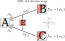
\includegraphics[draft=false, width=\linewidth]{qss/qss_distribution_stage}
		
	\end{subfigure}
	\begin{subfigure}{0.8\linewidth}
		\centering
		\caption{\label{fig:qss_encryption_stage}}
		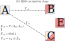
\includegraphics[draft=false, width=\linewidth]{qss/qss_encryption_stage}
		
	\end{subfigure}
\caption{\label{fig:qss_protocol_cartoon} Distribution and encryption stages of our QSS protocol. Alice (A) wishes to securely share her secret $\sigma_A$ amongst potentially dishonest recipients Bob (B) and Charlie (C). (a) Distribution stage. B and C send coherent states chosen from QPSK alphabet to Alice, who heterodynes and obtains outcomes $A_B, A_C$. Dishonest Eve will eavesdrop on the distribution of quantum states in order to gain information about $A_B, A_C$. (b) Encryption stage. Alice will form variable $X_A$ using her chosen function $\mathcal{F}$ with her heterodyne measurement outcomes as input variables. She converts $X_A$ to binary $\tilde{X}_A$ and encrypts the secret with it to reach $\varsigma_A = \sigma_A \oplus \tilde{X}_A$. The encrypted secret is then broadcast. Dishonest players are shown in red and honest players in gray. A combination of red and gray denotes uncertainty about dishonesty.
}
\end{figure}

Since Alice is the dealer who will decide on the eventual shared key our protocol is analogous to a reverse-reconciliation (RR) QKD system, and so we may similarly expect the performance benefits of RR QKD at high loss and noise. We note that having potentially untrusted players as the senders may open the protocol up to new classes of attack, for example if they are permitted to send a state which is outside the QPSK alphabet, and such attacks should be addressed in future work.

%\MT{talk somewhere about the types of attack we allow}


Our QSS protocol runs in three stages, a Distribution stage, an Encryption stage and, finally, a Decryption stage. Distribution and encryption stages are displayed in Fig.~\ref{fig:qss_protocol_cartoon}. The Distribution stage, Fig.~\ref{fig:qss_distribution_stage}, involves distribution and measurement of quantum coherent states chosen from QPSK alphabet. At the end of Distribution, Alice will hold classical information which is correlated with both Bob and Charlie. In the Encryption stage, Fig.~\ref{fig:qss_encryption_stage}, Alice will combine her classical information and use it to encode her sensitive classical secret. The encoded secret is distributed to Bob and Charlie. The secret is decoded by Bob and Charlie during Decryption. Our protocol setup is described in Fig.~\ref{fig:qss_structure},~\ref{fig:qss_protocol_cartoon}, and we describe it in detail below.

%\MT{make sure that the following is in the same style as my qds protocol description}

\subsubsection*{Distribution stage, Fig.~\ref{fig:qss_distribution_stage}}
\paragraph{Step $1$}
Alice wishes to encrypt a classical secret, $\sigma_A$. Bob forms a classical random variable $X_B = \left\{\phi_B\right\}$, where the $\phi_B$ are complex phases independently chosen from the QPSK alphabet. Phases $\phi_B$ are assumed to be chosen uniformly at random, but we relax this assumption in Chapter~\ref{chapter:aqc}. Charlie likewise forms classical random variable $X_C = \left\{\phi_C\right\}$.

\paragraph{Step $2$}
Bob and Charlie form sequences of coherent states based on their random variables
\begin{equation}
\rho\left[X_{\left(B, C\right)}\right] := \otimes \rho\left[\phi_{\left(B, C\right)}\right]
\end{equation}
where $\rho\left[\phi_{\left(B, C\right)}\right]$ denotes a coherent state with phase $\phi_{\left(B, C\right)}$. These sequences of states are sent to Alice through quantum channels. %\MT{Talk later about the types of channels which these are.}. 
Alice performs heterodyne detection, Sec.~\ref{sec:intro_heterodyne} on each of her received states and records her complex outcomes. We denote the strings of Alice's measurement outcomes as $A_B, A_C$, where $A_B$ corresponds to measurement outcomes from states sent by Bob, and $A_C$ corresponds to those on states sent by Charlie. The $A_B$ and $A_C$ are kept separate and secret, and Bob and Charlie should retain their information $X_B, X_C$.

\subsubsection*{Encryption stage, Fig.~\ref{fig:qss_encryption_stage}}

\paragraph{Step $3$} Alice creates a new string of complex variables
\begin{equation}
X_A = \mathcal{F}\left(A_B, A_C\right)
\end{equation}
from her measurement outcomes. The function $\mathcal{F}$ is chosen by Alice and should be freely chosen to optimize security. In this thesis we will pick simple forms for $\mathcal{F}$ which allow us to easily make concrete predictions about protocol security, although in general $\mathcal{F}$ may be as pathological as Alice desires.

% \MT{Where shall I talk about function $F$?} \MT{I can create some nice graphs of different functions $F$, even those requiring a lot of parameters to be optimized over. But when it comes to actually analysing security I should pick simple ones.} 

\paragraph{Step $4$} Alice now holds random variable $X_A$ of complex variables, which depends on both Bob and Charlie's choices $X_B, X_C$. Alice maps her string of complex variables onto a binary random variable $X_A \mapsto \tilde{X}_A$, and uses $\tilde{X}_A$ to encode $\sigma_A$ via an XOR operation. For ease we shall write this combined step in terms of an encryption function $\text{Enc}$, which should be known to all players at the start of the protocol. % I should probably talk about this later at some point?

\begin{equation}
\varsigma_A = \text{Enc}\left(\sigma_A, X_A\right)
\end{equation}

\noindent Alice distributes $\varsigma_A$ to Bob and Charlie, who are unable to access $\sigma_A$ since they do not yet know $X_A$.

\subsubsection*{Decryption stage}

\paragraph{Step $5$} Later, when Alice desires to allow Bob and Charlie access to $\sigma_A$, she broadcasts her choice of function $\mathcal{F}$, along with enough classical information to perform a reconciliation procedure between $X_A$ and $\mathcal{F}\left(X_B, X_C\right)$. This stage is similar to CV QKD and so we will not discuss it further. Bob and Charlie contribute their information $X_B, X_C$ to form $\mathcal{F}\left(X_B, X_C\right)$ and reconcile it to $X_A$ and thus $\tilde{X}_A$. Then they are able to access Alice's original secret $\sigma_A$.

Critical to the protocol is the fact that Alice forms a secret key based on a degree of freedom shared between Bob and Charlie, which forces collaboration. In this way, our protocol is a natural extension of the protocol from Kogias \emph{et. al.} \cite{Kogias2017}, and may be seen to help bridge the gap betwee entanglement-based and sequential QSS.

If either one of Bob or Charlie is dishonest, they are forced to work with an honest player and so our scheme has succeeded.



%\MT{some more remarks about the running of the protocol}


\section{Security against Eve}\label{sec:qss_honest_recipients}
%\MT{talk here about security against an external eavesdropper.}

The QSS protocol presented above must be secure against both the actions of an external eavesdropper and those of a dishonest Bob or Charlie who may be collaborating with Eve. We will first consider security against Eve in order to illustrate key steps from the security analysis, and so for this section we assume that Bob and Charlie are honest,
Fig.~\ref{fig:qss_honest_recipients}. In Sec.~\ref{sec:qss_dishonest_recipient} we will begin to allow for dishonesty in recipients Bob and Charlie.

\begin{figure}[htp]
\centering
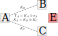
\includegraphics[draft=false, width=0.4\linewidth]{qss/qss_honest_recipients}
\caption{\label{fig:qss_honest_recipients} Alice will distribute her secret $\sigma_A$ to Bob and Charlie who are assumed honest. Dishonest Eve will try to attack the protocol and gain information about $\sigma_A$. Gray: honest. Red: dishonest. See Fig.~\ref{fig:qss_structure} for further information.}
\end{figure}


The starting point for our security analysis is the following Devetak-Winter bound \cite{Devetak2004} for the asymptotic key rate under collective attack, Fig.~\ref{fig:types_of_attack_collective},

%\MT{should I motivate why this bound is helpful for us?}

\begin{equation}\label{eqn:qss_dw_eve}
\kappa_{\text{Eve}} \ge \text{I}\left(X_A : X_B, X_C\right) - \chi\left(X_A : \mathbb{E}\right)
\end{equation}

\noindent which describes the balance between the mutual information, $\text{I}$, shared between Alice and a Bob-Charlie collaboration, and the Holevo information $\chi$ between Eve's quantum system $\mathbb{E}$ and Alice. It is perhaps unsurprising that Eq.~\ref{eqn:qss_dw_eve} should be our starting point given the noted similarities between QSS and QKD. The $X_A = \mathcal{F}\left(A_B, A_C\right)$ is Alice's variable based on her heterodyne measurement outcomes.

We would like to calculate the lower bound for key rate given by Eq.~\ref{eqn:qss_dw_eve} and so we will consider each term in turn and demonstrate how they may be calculated for the protocol described above.



\subsection{Mutual information}

Using Eq.~\ref{eqn:intro_mutual_information} the mutual information $\text{I}$ may be written as 
\begin{equation}\label{eqn:qss_deriv_1}
\text{I}\left(X_A : X_B, X_C\right) = \text{H}\left(X_B, X_C\right) - \text{H} \left(X_B, X_C \given X_A\right).
\end{equation}
where the first term on the right hand side is the joint Shannon entropy of $X_B$ and $X_C$, and the second term is the conditional Shannon entropy of $X_B, X_C$ given $X_A$, Sec.~\ref{sec:intro_shannon_entropy}. Intuitively this second term encodes the uncertainty one has about which $X_B, X_C$ were chosen, once Alice has formed $X_A$, while the first term encodes the \emph{a priori} entropy about Bob and Charlie's choice of sent coherent states.

The joint Shannon entropy may be written
\begin{equation}\label{eqn:qss_deriv_2}
\text{H}\left(X_B, X_C\right) = \sum_{X_B=b, X_C=c} - \text{P}\left(b, c\right) \log \text{P}\left(b, c\right)
\end{equation}
where $b, c$ are individual instances of variables $X_B, X_C$. In the following we shall take $b, c$ as phase elements of the QPSK alphabet, but this may be readily generalized to an $N$PSK alphabet. 

Since $b, c$ are taken to be independently chosen and uniformly random we see that the joint probability
\begin{equation}\label{eqn:qss_deriv_3}
\text{P}\left(b, c\right) = \text{P}\left(b\right)\times \text{P}\left(c\right) = \frac{1}{16}
\end{equation}
since each of the $b, c$ are chosen with probability $1/4$. We will relax this assumption in Chapter~\ref{chapter:aqc}.

Expanding the conditional entropy in $X_A$ via Eq.~\ref{eqn:intro_conditional_entropy_expansion} \cite{Wilde2013} we reach

\begin{equation}\label{eqn:qss_deriv_4}
\text{H}\left(X_B, X_C \given X_A\right) = \int\limits_{a \in \mathbb{C}} \Diff2 a \; \text{P}\left(X_A = a\right) \text{H}\left(X_B, X_C \given X_A = a\right),
\end{equation}
and we shall see that each term in Eq.~\ref{eqn:qss_deriv_4} can be calculated once function $\mathcal{F}$ is known. The conditional entropy $\text{H}\left(X_B, X_C \given X_A = a\right)$ expands as 

\begin{align}
\text{H}\left(X_B, X_C \given X_A=a\right) = - \sum_{b, c}  &\text{P}\left(X_B=b, X_C=c \given X_A=a\right) \times \notag \\
%
&\log \text{P}\left(X_B=b, X_C=c \given X_A=a\right) \label{eqn:qss_deriv_4_1}
\end{align}

\noindent and so all that remains is to calculate the probabilities 
\begin{align}
\label{eqn:qss_prob1} \text{P}\left(X_A=a\right) \qq{and} \\
\label{eqn:qss_prob2} \text{P}\left(X_B=b, X_C=c \given X_A=a\right)
\end{align}
with respect to a given function $\mathcal{F}$.


\subsubsection{Function $\mathcal{F}$}


We have no requirement that $\mathcal{F}$ should be injective. This implies, for example, that $\text{S}\left(\rho_{\left.\mathbb{E} \given A_B, A_C\right.}\right) \ne \text{S}\left(\rho_{\left. \mathbb{E} \given X_A\right.}\right)$, i.e. the entropy of Eve's quantum state conditioned on Alice's heterodyne outcomes $A_B, A_C$ is not equal to the entropy of Eve's quantum state conditioned on Alice's variable $X_A$, and so we must carefully consider the action of $\mathcal{F}$ early on in our analysis. 

To be concrete, in what follows we assume that $F$ is linear
\begin{equation}\label{eqn:qss_F_linear}
\mathcal{F}\left(x, y\right) := g x + h y \qq{with} g, h \in \mathbb{R}\setminus \left\{0\right\}
\end{equation} 
which will enable us to make some predictions about the performance of the protocol. Although we make no claims about the optimality of this choice of $\mathcal{F}$, we are free to optimize the key rate over $g, h$, and we will make it clear when we have done so. In Sec.~\ref{appendix:qss_moreF} we consider some alternative forms for $\mathcal{F}$.





\subsubsection{Expanding classical probabilities}

Applying Bayes' formula Eq.~\ref{eqn:intro_bayes} to probability Eq.~\ref{eqn:qss_prob2} we see that
\begin{align}
\text{P}\left(X_B=b, X_C=c \given X_A=a\right) = \text{P}&\left(X_A=a \given X_B=b, X_C=c\right) \notag \\
&\times \frac{\text{P}\left(X_B=b, X_C=c\right)}{\text{P}\left(X_A=a\right)}.
\end{align}


\noindent Now, we can access $\text{P}\left(X_A=a \given X_B=b, X_C=c\right)$. 
%by modelling the effects of the channel on quantum states distributed by Bob and Charlie. 
We take
\begin{equation}\label{eqn:qss_deriv_5}
X_A = \mathcal{F}\left(A_B, A_C\right) = g A_B + h A_C
\end{equation}
as in Eq.~\ref{eqn:qss_F_linear} and so we rearrange
\begin{equation}
A_C = \frac{X_A - g A_B}{h}.
\end{equation}

\noindent Since our $F$ is not injective %(there are multiple $A_B, A_C$ which will give the same $X_A$)
we must average over all of the possible ways to reach a given $X_A$. Therefore, once $X_A, g$ and $h$ are fixed, the choice of $A_B, A_C$ reduces to a one-variable problem. So

\begin{equation}\label{eqn:qss_deriv_5_1}
\text{P}\left(X_A \given X_B=b, X_C=c\right) = \int\limits_{A_B \in \mathbb{C}} \Diff2 A_B \; \text{P}\left(A_B , \frac{X_A - g A_B}{h} \given X_B=b, X_C=c\right)
\end{equation}
which may be calculated once we know how the channel acts on input states. Note that an analogous expression would be reached by rearranging Eq.~\ref{eqn:qss_deriv_5} as $A_B = \left(X_A - h A_C\right)/g$, but it will make no difference to the resulting quantities which we derive from Eq.~\ref{eqn:qss_deriv_5_1}

Assuming that the two channels, one from Charlie$\rightarrow$Alice and one from Bob$\rightarrow$Alice, are independent from each other\footnote{We shall see later what this means for their combined action on an input quantum state} allows us to write
\begin{equation}\label{eqn:qss_deriv_6}
\text{P}\left(A_B, A_C \given X_b=b, X_C=c\right) = \text{P}\left(A_B \given X_B=b\right) \times \text{P}\left(A_C \given X_C=c\right)
\end{equation}
for the probabilities that Alice's heterodyne measurement outcomes are $A_B, A_C$ if coherent states with phases $\phi_B = b, \phi_C = c$ are sent.

Let us assume for now that each channel is noiseless but lossy. The probability that Alice measures a particular heterodyne outcome $a \in \mathbb{C}$ when a coherent state of complex amplitude $\beta$ is sent through a lossy channel, transmittivity $T$, is (Sec.~\ref{sec:qss_perr}) %where do I actually derive this? I should put it in one place and then refer to it a bunch
\begin{equation}\label{eqn:qss_channel_classical_prob}
\text{P}\left(a \given \beta, T\right) = \frac{1}{\pi}\exp\left( - \left| a - \sqrt{T}\beta \right|^2\right)
\end{equation}
which we have used previously in Ch.~\ref{chapter:qds}. The required changes to include thermal noise of the channel can be readily made, Sec.~\ref{sec:thermal_channel}.

The integral in Eq.~\ref{eqn:qss_deriv_5_1} may be calculated analytically to reach 
\begin{align}\label{eqn:qss_deriv_7}
\text{P}\left(X_A \given X_B=b, X_C=c\right) = \frac{1}{\pi} \frac{1}{g^2 + h^2} &\exp \left( - \frac{\left[b^R g \sqrt{T_B} + c^R h \sqrt{T_C} - X_A^R \right]^2}{g^2 + h^2}\right) \notag \\
%
&\times \exp \left( - \frac{\left[b^I g \sqrt{T_B} + c^I h \sqrt{T_C} - X_A^I \right]^2}{g^2 + h^2} \right)
\end{align}
where $b, c$ are Bob and Charlie's coherent state amplitudes, $X_A$ is Alice's final variable after applying $\mathcal{F}$ Eq.~\ref{eqn:qss_F_linear} to her heterodyne outcomes, $T_B, T_C$ are the transmittivities of the Bob$\rightarrow$Alice channel and Charlie$\rightarrow$Alice channel, respectively, and a superscript $R\left(I\right)$ denotes the real (imaginary) part of the corresponding quantity. %\MT{I probably don't need to say much about how this integration is actually done, since it should be obvious.} 
The probability $\text{P}\left(X_A=a\right)$ Eq.~\ref{eqn:qss_prob1} may now be found by %summing Eq.~\ref{eqn:qss_deriv_7} over all $b, c$ in our QPSK alphabet.

\begin{equation}\label{eqn:qss_deriv_pxa}
\text{P}\left(X_A\right) = \sum_{b, c} \text{P}\left(X_A \given X_B=b, X_C=c\right).
\end{equation}






Finally, the mutual information Eq.~\ref{eqn:qss_deriv_1} may be calculated. We perform the integration over $X_A$ in Eq.~\ref{eqn:qss_deriv_4} numerically and display the mutual information $I$ in Fig.~\ref{fig:qss_mutinf_graphs}.


% Have some graphs of the various probabilities and mutual information


%Let us now explore how the mutual information behaves. \MT{Now let's make some graphs and really have fun exploring how $I$ behaves.}

\subsection{Holevo information}

We will now detail how the Holevo information term in Eq.~\ref{eqn:qss_dw_eve} may be calculated. In doing so we will point to areas where future work might strengthen the security analysis to consider wider classes of attack, which should illuminate the contexts to which our security proof may be applied. In this section we consider a dishonest Eve performing attack BS$0$, as detailed above in Sec.~\ref{sec:qds_bs0}, though the analysis follows readily for the other attacks described in Sec.~\ref{sec:qds_attack_analysis}. We will then compare the strength of attacks BS$0$, BS$1$, BS$2$ and EC. % and more general attacks will be considered later.

Bob and Charlie prepare a state from the QPSK alphabet, and each state is chosen randomly and with equal probability. Before the channel, Bob and Charlie hold the joint state
\begin{equation}
\rho_{\text{before}} = \rho_B \otimes \rho_C
\end{equation}
with
\begin{equation}
\rho_B = \frac{1}{4} \sum_{k=0}^3 \dyad{\beta_k}_B \qq{and} \rho_C = \frac{1}{4} \sum_{k^\prime = 0}^3 \dyad{\gamma_{k^\prime}}_C
\end{equation}
where $\beta, \gamma$ are the amplitudes of Bob's and Charlie's coherent state alphabets.\footnote{These complex amplitudes $\beta, \gamma$ were denoted $b, c$ in the previous section.}

We assume that the channel acts separately on each mode, and that modes $\rho_B$, $\rho_C$ undergo independent evolution. In other words, we assume that the channel has the following structure
\begin{equation}\label{eqn:qss_channel}
\Phi\left[\rho\right] = \Phi_B\left[\rho\right] \otimes \Phi_C\left[\rho\right]
\end{equation}
where $\Phi_{B, C}$ denote the lossy channels described by attack BS$0$, Sec.~\ref{sec:qds_bs0}, and the subscript $B, C$ denotes which mode of $\rho_{\text{before}}$ each channel acts on. 
\iffalse
\begin{align}
\Phi_B\left[\rho\right] = \varphi_B\left(\text{Tr}_C \rho\right) \otimes \mathds{1}_C\left(\text{Tr}_B\rho\right) \notag \\
\Phi_C\left[\rho\right] = \mathds{1}_B\left(\text{Tr}_C\rho\right) \otimes \varphi_C\left(\text{Tr}_B\rho\right)
\end{align}
with $\mathds{1}$ the identity channel and $\varphi_{B,C}$ denotes the lossy channels described by attack BS$0$, Sec.~\ref{sec:qds_bs0}. The Total 
\fi
The total channel $\Phi$ preserves the tensor-product structure of the input state.

Physically $\Phi$ corresponds to the case where Eve performs separate beamsplitter attacks on each channel and retains two output modes $\mathbb{E}_{B, C}$, Fig.~\ref{fig:qss_bs0_attack}.

\begin{figure}[htp]
\centering
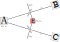
\includegraphics[draft=false, width=0.8\linewidth]{qss/qss_bs0}
\caption{\label{fig:qss_bs0_attack} We model the channel $\Phi$ as two independent beamsplitter attacks of type BS$0$, Sec.~\ref{sec:qds_bs0}. This preserves the tensor-product structure of $\rho_{\text{before}}$.}
\end{figure}


The total state after the channel becomes
\begin{equation}
\rho_{\text{after}} = \rho_{\mathbb{A}_B, \mathbb{E}_B} \otimes \rho_{\mathbb{A}_C, \mathbb{E}_C}
\end{equation}
with $\mathbb{A}_{B, C}$ denoting Alice's two modes and where
\begin{equation}
\rho_{\mathbb{A}_B, \mathbb{E}_B} = \frac{1}{4} \sum_{k=0}^3 \dyad{\sqrt{T_B} \beta_k}_{\mathbb{A}_B} \otimes \dyad{\sqrt{1-T_B} \beta_k}_{\mathbb{E}_B}
\end{equation}
and similarly for $\rho_{\mathbb{A}_C, \mathbb{E}_C}$. Now, Alice heterodynes and measures $A_B \in \mathbb{C}$ from $\rho_{\mathbb{A}_B, \mathbb{E}_B}$ and $A_C \in \mathbb{C}$ from $\rho_{\mathbb{A}_C, \mathbb{E}_C}$. Eve's total state conditioned on these outcomes becomes 
\begin{equation}\label{eqn:qss_eve_conditional}
\rho_{\left.\mathbb{E} \given A_B, A_C\right.} = \rho_{\left.\mathbb{E}_B \given A_B\right.} \otimes \rho_{\left. \mathbb{E}_C \given A_C\right.}
\end{equation}
with
\begin{equation}
\rho_{\left.\mathbb{E}_B \given A_B\right.} = \frac{1}{4 \pi} \sum_{k=0}^3 \text{P}_B\left(A_B \given \beta_k, T_B\right) \dyad{\sqrt{1-T_B} \beta_k}_{\mathbb{E}_B}
\end{equation}
and similarly for $\rho_{\left.\mathbb{E}_C \given A_C\right.}$. The probability $\text{P}_B\left(A_B \given \beta_k, T_B\right)$ is calculated analogously to Eq.~\ref{eqn:qss_channel_classical_prob}, and similarly for $A_C$.

To proceed, we take $X_A = g A_B + h A_C$ as usual, with $g, h$ fixed, and write $A_C = \left(X_A - g A_B\right)/h$. Therefore the state $\rho_{\left.\mathbb{E} \given A_B, A_C\right.}$, Eq.~\ref{eqn:qss_eve_conditional}, becomes

\begin{align}\label{eqn:qss_deriv_8}
\rho_{\left. \mathbb{E} \given X_A, A_B\right.} &= \frac{1}{16 \pi^2} \sum_{k, k^\prime = 0}^3 \text{P}_B\left(A_B \given \beta_k, T_B\right) \text{P}_C\left(\frac{X_A - g A_B}{h} \given \gamma_{k^\prime}, T_C\right) \notag \\
%
&\dyad{\sqrt{1-T_B} \beta_k}_{\mathbb{E}_B} \otimes \dyad{\sqrt{1-T_C}\gamma_{k^\prime}}_{\mathbb{E}_C}
\end{align}

\noindent Once again since Alice's function $\mathcal{F}$ is in general not injective we must mix over outcomes $A_B, A_C$ in order to find Eve's state $\rho_{\left.\mathbb{E} \given X_A\right.}$. Therefore 

\begin{equation}\label{eqn:qss_aposteriori_state}
\rho_{\left.\mathbb{E} \given X_A\right.} = \int\limits_{A_B \in \mathbb{C}} \Diff2 A_B \; \text{P}\left(A_B\right) \rho_{\left.\mathbb{E} \given X_A, A_B\right.}
\end{equation}

\noindent and mixing over $X_A$ we finally reach

\begin{equation}\label{eqn:qss_apriori_state}
\rho_{\mathbb{E}} = \int\limits_{X_A \in \mathbb{C}} \Diff2 X_A \; \text{P}\left(X_A\right) \rho_{\left.\mathbb{E}\given X_A\right.}.
\end{equation}

\noindent We may identity Eq.~\ref{eqn:qss_aposteriori_state} as Eve's \emph{a prosteriori} state and Eq.~\ref{eqn:qss_apriori_state} as Eve's \emph{a priori} state and so Eve's Holevo information is given by the usual formula

\begin{equation}\label{eqn:qss_holevo}
\chi = \text{S}\left(\rho_\mathbb{E}\right) - \int\limits_{X_A \in \mathbb{C}} \Diff2 X_A \; \text{P}\left(X_A\right) \text{S}\left(\rho_{\left.\mathbb{E} \given X_A\right.}\right).
\end{equation}
where we note that we can no longer simplify the second term in Eq.~\ref{eqn:qss_holevo}, as we did in Sec.~\ref{sec:qds_attack_analysis}, for example, since in general each state $\rho_{\left.\mathbb{E} \given X_A\right.}$ will have a different entropy.


\noindent Let us explore the behaviour of Eve's Holevo information Eq.~\ref{eqn:qss_holevo}.

\MT{TODO: make some nice graphs of $\chi$ in different scenarios and under different attacks BS1, BS2, EC.}

\section{Security against a dishonest player}
%\MT{Talk about guarding against a dishonest Bob/Charlie.}
Of course, if Alice only had to guard against an external Eve, and both Bob and Charlie could be assumed honest, then the QSS task becomes much easier. She could, for example, simply send the same information to each recipient. Or send her secret just to the recipient she is interested in, with no need to ``split'' it or share it. 

\subsection{Dishonest Bob}
Let us translate the analysis from Sec.~\ref{sec:qss_honest_recipients} to the case where either Bob or Charlie is dishonest, but Alice does not know which one, Fig.~\ref{fig:qss_structure}. Including a dishonest recipient in the above security proof requires us to re-calculate several quantities. For concreteness we will first assume that Bob is dishonest and Charlie is honest, Fig.~\ref{fig:qss_dishonest_Bob}, and we will allow Bob to collaborate with Eve. Later we will discuss how to account for the fact that we do not know \emph{which} player is dishonest.

\begin{figure}[htp]
\centering
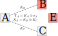
\includegraphics[draft=false, width=0.6\linewidth]{qss/qss_dishonest_Bob}
\caption{\label{fig:qss_dishonest_Bob} A dishonest Bob gains an advantage since he knows which coherent state he chose to send to Alice. He may additionally choose to collaborate with Eve in order to gain information about Alice's measurement on Charlie's state. c.f. Fig.~\ref{fig:qss_structure}.}
\end{figure}

The main effect of permitting dishonesty from Bob is that he knows precisely which coherent states he sent to Alice. This will give him reduced uncertainty about Alice's variable $X_A$. Bob might also wait and see which coherent state was sent by Charlie before choosing his own, in order to preference a certain outcome $X_A$. \MT{Make some comments about this.} We will assume that Bob sends states only from the QPSK alphabet, though in principle this could be relaxed in future work.

Since Bob knows which coherent states he sent we must re-calculate several expressions from Sec.~\ref{sec:qss_honest_recipients} with the key change that we no longer mix over Bob's alphabet. The quantities which this influences are

\begin{equation}
\text{P}\left(X_A=a\right) = \sum_{c} \text{P}\left(X_A \given X_b=b, X_C=c\right)
\end{equation}

\noindent and

\begin{align}
\text{H}\left(X_B, X_C \given X_A=a\right) = - \sum_{c} \text{P}&\left(X_B=b, X_C=c \given X_A=a\right) \times \notag \\
&\log \text{P}\left(X_B=b, X_C=c \given X_A=a\right)
\end{align}

\noindent and the mutual information may now be calculated as in the previous section. 

The Holevo information is also calculated analogously to the previous section, the key change being that Eve's state conditioned on $X_A, A_B$, Eq.~\ref{eqn:qss_deriv_8}, is now given by
\begin{align}\label{eqn:qss_deriv_9}
\rho_{\left.\mathbb{E} \given X_A, A_B\right.} &= \frac{1}{4 \pi^2} \sum_{k^\prime=0}^3 \text{P}_B\left(A_B \given \beta_k, T_B\right) \text{P}_C\left(\frac{X_A - g A_B}{h} \given \gamma_{k^\prime}, T_C\right) \notag \\
%
&\dyad{\sqrt{1-T_B} \beta_k}_{\mathbb{E}_B} \otimes \dyad{\sqrt{1-T_C}\gamma_{k^\prime}}_{\mathbb{E}_C}
\end{align}
and the \emph{a posteriori} and \emph{a priori} states calculated by integrating Eq.~\ref{eqn:qss_deriv_9} identically to Eqs.~\ref{eqn:qss_aposteriori_state},~\ref{eqn:qss_apriori_state}.

Since we no longer mix over Bob's coherent state $b$, the mutual information $\text{I}$ and Holevo information $\chi$ have become functions of $b$. In this chapter we assume that each state in the QPSK alphabet is equally likely and has equal magnitude and so both $\text{I}$ and $\chi$ will be identical for each of Bob's alphabet states. We will relax this in Chapter~\ref{chapter:aqc}.


The final key rate is now
\begin{equation}\label{eqn:qss_keyrate_dishonest_Bob}
\kappa_{\text{Eve, Bob}} = \text{I}\left(X_A : X_B, X_C\right) - \chi\left(X_A : \mathbb{E} \mathbb{B}\right)
\end{equation}
with mutual information and Holevo information terms calculated as described above.


%\MT{Make some graphs of things with dishonest Bob}


\subsection{Dishonest Bob or Dishonest Charlie}
If Alice is certain that Bob is the dishonest player then she has no need for a secret sharing scheme. Equivalently, she can set $g=0$ in her function $\mathcal{F}$. If she is correct about Bob's dishonestly, then she has successfully prevented him from gaining any information about her secret. However, if Alice turns out to be wrong and it is Charlie who is the dishonest player then she has accidentally given Charlie the secret! It is the uncertainty about which player is dishonest which makes a QSS scheme necessary.

In order to take into account this uncertainty over which player is dishonest, Fig.~\ref{fig:qss_structure}, we proceed as in the recent QSS works Refs.~\cite{Kogias2017, Grice2019} and calculate the minimum over all possible dishonest configurations. That is, we take

\begin{equation}
\kappa \ge \min \left\{\kappa_{\text{Eve, Bob}}, \kappa_{\text{Eve, Charlie}}\right\}
\end{equation}
where $\kappa_{\text{Eve, Charlie}}$ is calculated analogously to Eq.~\ref{eqn:qss_keyrate_dishonest_Bob}. \MT{Comment about why this works.}


\section{Protocol performance}
\MT{Make some graphs of key rate and tweak all of the parameters that I can in all of the attacks that I can.}

\MT{If I have time, make some graphs with e.g. homodyning instead of heterodyning, or different alphabets.}

















\section{Outlook}
%\MT{this section should be somewhere else, perhaps in an "outlook" section?}
The classical post-processing of the above protocol is inherently very similar to Ref.~\cite{Kogias2017}, in which a secret key is generated between Alice and a shared Bob-Charlie degree of freedom via incompatible homodyne measurements on a tripartite entangled state. We expect that our protocol will be secure against a more restricted set of attacks, but over a wider range of channel parameters, for several reasons. 

Firstly unlike Ref.~\cite{Kogias2017} which relies in generation and distribution of large multipartite entangled states, our scheme has much more modest quantum requirements which are known to be easy to generate and manipulate, and which will be much more robust to channel loss and channel noise than a large entangled state. Quantum cryptography using continuous-variables typically operates over metropolitan distances of tens of kilometers, and so we might reasonably expect similar performance of our QSS protocol. Performance of our protocol over a realistic fiber channel is analysed in Chapter~\ref{chapter:aqc}. 

Secondly, the protocol from Ref.~\cite{Kogias2017} takes a form analogous to direct-reconciliation (DR) QKD, while ours is analogous to reverse-reconciliation (RR) QKD. RR QKD is known \cite{Grosshans2002, Grosshans2003, Laudenbach2017} to be much more resilient to loss and noise than DR QKD without modifications \cite{Silberhorn2002}.

Ref.~\cite{Kogias2017} has potentially dishonest players Bob and Charlie performing homodyne measurements on incompatible observables (i.e. switching between $q$ and $p$ quadratures). No assumptions are made about the measurement devices used and they are each treated as a "black-box". Security comes inherently because of a Heisenberg-type relation between incompatible observables, and the security proof relies on an Entropic Uncertainty Relation (EUR) whic hhave had success in many parts of quantum cryptography \cite{Furrer2012, Furrer2017}. However, since we desire to use heterodyne detection we are forced to adopt a different approach and explicitly model the states' evolution and measurement during the protocol. We note that this matches the current state-of-the-art of QPSK-based QKD \cite{Papanastasiou2018}, but should be improved in future work.

We have assumed that a dishonest Bob or Charlie still sends a state from the QPSK alphabet. It is yet unclear whether they could gain an advantage by sending something exotic and potentially highly entangled, perhaps in order to force Alice to reach a certain key $X_A$. This should be explored and potentially relaxed in future work. We anticipate that applying methods from quantum bit commitment \cite{Broadbent2015} might prove fruitful here, since bit commitment also relies on a potentially dishonest distribution of the quantum state.

Finally, we note that our assumption that the channel between Alice and Bob-Charlie takes a tensor-product structure, Eq.~\ref{eqn:qss_channel}, Fig.~\ref{fig:qss_bs0_attack} is a strong one and should be relaxed. A potential strategy of a dishonest player could be to exploit properties of a general channel which maps a two-mode input state to a two-mode output state at Alice, potentially allowing a dishonest player many output ancilla modes correlated with Alice. Such a strategy will be restricted by the conditions that the reduced state of an honest player should be a coherent state (with noise). Similarly it will require that Alice's measurement outcomes don't look ``too errant'', though this should be quantified.









\chapter{Agile quantum cryptography}
Goal of chapter: introduce and make explicit the concept of quantum agility in quantum cryptography. Join together several threads from the previous two chapters. This chapter can be viewed as a "bonus" to the QDS and QSS chapters.

\iffalse
Key things I want to present, in roughly the order that I want to present them:

\begin{itemize}
\item Discussion of agility and why it might be desirable. Motivate it in terms of my two literature reviews.
\item Modification of QDS protocol from earlier to be agile with QSS (i.e. introduce protocol QSS-b and prove its security (inc postselection)). Have some graphs of its behaviour
\item Bring in QKD from the literature (Papanastasiou2018). Have some graphs of its behaviour and discussion of how it relates to my thesis.
\item Talk about the experiment (emphasise that it is not my work). I can have some plots of raw data (opendata), and make graphs of data points which I received.
\item Analysis of the data under each protocol with discussion of how results from previous chapters are modified to make them more realistic
\item Graphs of performance at different data parameters
\item Table from the AQC paper $\leftarrow$ this can be the climax of this section
\item star graph of QDS
\item Discussion of how our analysis motivates agility
\item Outlook/next steps
\end{itemize}
\fi

\section{Introduction}

% Review some things from my previous two literature reviews
We have observed over the past two chapters, and in our overviews of quantum cryptography in Chapter~\MT{X}, that several quantum cryptographic protocols are intimately related. As Simmons noted

\MT{insert simmons quote}

and so we have seen close connections between QKD and QSS, and QSS may be interpreted simply as QKD performed between one player (dealer) and several players (recipients of the secret). We have also remarked that the secret sharing task may be performed pseudo-classically, by first encrypting channels using QKD and then using an unconditionally secure classical secret sharing protocol. 

It was noted \MT{cite some papers} that QSS is related to quantum conferencing and often the same hardware setup may be used to perform both tasks. And in Ref.~\MT{cite} it was explicitly demonstrated that a round-robin QSS protocol can also be used to perform QKD between any two players. Moving to the QDS literature, ever since discovery of practical QDS requiring neither quantum memory, entanglement or an optical multiport that there are close links between QDS and QKD. Ref.~\MT{cite} explicitly builds their QDS protocol to use QKD hardware, while Ref.~\MT{cite} realise a setup which can, with minimal hardware modification, perform either QDS or QKD, with additional MDI capabilities. And in Refs.~\MT{cite a bunch of stuff} it was explicitly remarked that QDS differs from QKD \emph{only} in the classical postprocessing. Finally, in Ref.~\MT{cite} the authors design their QSS scheme on the same principles as DPS QKD \MT{define and check}. And many papers build their security proofs on techniques designed for QKD \MT{cite loads of stuff.}

%We therefore might ask 

It should be clear that the field of quantum cryptography is far broader than mere QKD. As we move closer towards practical implementation of diverse quantum cryptographic protocols we must consider not only the unconditional security of the underlying protocol, but also its ease of implementation. As protocols are designed with minimal and often overlapping hardware requirements we may ask the question:
\\
\par
\emph{given a particular hardware setup, which quantum protocols can I perform?}
\\
\\
\noindent Or, desiring a large-scale quantum cryptographic network:
\\
\par
\emph{given a deployed network architecture, which quantum protocols can I perform with minimal disruption?}
\\
\\
\noindent Both of these questions have deep impacts on the success probability of a future large-scale quantum network. \MT{Chat more about the networks. Mention DV over installed fibers results from recent years. (Did they require dedicated hardware?)}

We have already even seen several quantum routes to accomplishment of the same task. By first utilizing QKD between all players it is possible to perform DS \MT{cite} or SS \MT{cite} using unconditionally secure classical algorithms, and indeed this may often be preferable to protocols requiring large entangled states \MT{cite}. Alternatively, in a distributed quantum computing setup which can easily generate and distribute entanglement, a protocol such as Ref.~\MT{cite} may be advantageous if it takes advantage of already accessible hardware. 






%\part{Coherent signal transfer}
\end{document}